% This is "sig-alternate.tex" V2.1 April 2013
% This file should be compiled with V2.5 of "sig-alternate.cls" May 2012
%
% This example file demonstrates the use of the 'sig-alternate.cls'
% V2.5 LaTeX2e document class file. It is for those submitting
% articles to ACM Conference Proceedings WHO DO NOT WISH TO
% STRICTLY ADHERE TO THE SIGS (PUBS-BOARD-ENDORSED) STYLE.
% The 'sig-alternate.cls' file will produce a similar-looking,
% albeit, 'tighter' paper resulting in, invariably, fewer pages.
%
% ----------------------------------------------------------------------------------------------------------------
% This .tex file (and associated .cls V2.5) produces:
%       1) The Permission Statement
%       2) The Conference (location) Info information
%       3) The Copyright Line with ACM data
%       4) NO page numbers
%
% as against the acm_proc_article-sp.cls file which
% DOES NOT produce 1) thru' 3) above.
%
% Using 'sig-alternate.cls' you have control, however, from within
% the source .tex file, over both the CopyrightYear
% (defaulted to 200X) and the ACM Copyright Data
% (defaulted to X-XXXXX-XX-X/XX/XX).
% e.g.
% \CopyrightYear{2007} will cause 2007 to appear in the copyright line.
% \crdata{0-12345-67-8/90/12} will cause 0-12345-67-8/90/12 to appear in the copyright line.
%
% ---------------------------------------------------------------------------------------------------------------
% This .tex source is an example which *does* use
% the .bib file (from which the .bbl file % is produced).
% REMEMBER HOWEVER: After having produced the .bbl file,
% and prior to final submission, you *NEED* to 'insert'
% your .bbl file into your source .tex file so as to provide
% ONE 'self-contained' source file.
%
% ================= IF YOU HAVE QUESTIONS =======================
% Questions regarding the SIGS styles, SIGS policies and
% procedures, Conferences etc. should be sent to
% Adrienne Griscti (griscti@acm.org)
%
% Technical questions _only_ to
% Gerald Murray (murray@hq.acm.org)
% ===============================================================
%
% For tracking purposes - this is V2.0 - May 2012

\documentclass{sig-alternate-05-2015}


%Numbered environment
\newtheorem{SampleEnv}{Example}[section]
\newtheorem{theorem}{Theorem}
\newtheorem{lemma}{Lemma}

\begin{document}

% Copyright
\setcopyright{acmcopyright}
%\setcopyright{acmlicensed}
%\setcopyright{rightsretained}
%\setcopyright{usgov}
%\setcopyright{usgovmixed}
%\setcopyright{cagov}
%\setcopyright{cagovmixed}


% DOI
\doi{10.475/123_4}

% ISBN
\isbn{123-4567-24-567/08/06}

%Conference
\conferenceinfo{PLDI '13}{June 16--19, 2013, Seattle, WA, USA}

\acmPrice{\$15.00}

%
% --- Author Metadata here ---
\conferenceinfo{WOODSTOCK}{'97 El Paso, Texas USA}
%\CopyrightYear{2007} % Allows default copyright year (20XX) to be over-ridden - IF NEED BE.
%\crdata{0-12345-67-8/90/01}  % Allows default copyright data (0-89791-88-6/97/05) to be over-ridden - IF NEED BE.
% --- End of Author Metadata ---

\title{A New Algorithm To Evaluate Terminal Heads Of Length K }

%
% You need the command \numberofauthors to handle the 'placement
% and alignment' of the authors beneath the title.
%
% For aesthetic reasons, we recommend 'three authors at a time'
% i.e. three 'name/affiliation blocks' be placed beneath the title.
%
% NOTE: You are NOT restricted in how many 'rows' of
% "name/affiliations" may appear. We just ask that you restrict
% the number of 'columns' to three.
%
% Because of the available 'opening page real-estate'
% we ask you to refrain from putting more than six authors
% (two rows with three columns) beneath the article title.
% More than six makes the first-page appear very cluttered indeed.
%
% Use the \alignauthor commands to handle the names
% and affiliations for an 'aesthetic maximum' of six authors.
% Add names, affiliations, addresses for
% the seventh etc. author(s) as the argument for the
% \additionalauthors command.
% These 'additional authors' will be output/set for you
% without further effort on your part as the last section in
% the body of your article BEFORE References or any Appendices.

%\numberofauthors{8} %  in this sample file, there are a *total*
% of EIGHT authors. SIX appear on the 'first-page' (for formatting
% reasons) and the remaining two appear in the \additionalauthors section.
%
\author{
% You can go ahead and credit any number of authors here,
% e.g. one 'row of three' or two rows (consisting of one row of three
% and a second row of one, two or three).
%
% The command \alignauthor (no curly braces needed) should
% precede each author name, affiliation/snail-mail address and
% e-mail address. Additionally, tag each line of
% affiliation/address with \affaddr, and tag the
% e-mail address with \email.
%
% 1st. author
\alignauthor
David Pager\\
       \affaddr{Department of Information and Computer Science}\\
       \affaddr{University of Hawaii at Manoa}\\
       \email{pagerd@hawaii.rr.com}
% 2nd. author
\alignauthor
Xin Chen\\
       \affaddr{Department of Information and Computer Science}\\
       \affaddr{University of Hawaii at Manoa}\\
       \email{chenx@hawaii.edu}
}



\maketitle
\begin{abstract}
This paper presents a new FIRST$_k$($\alpha$) algorithm for finding
the terminal heads of length $k$ of a given string in a contextfree
grammar, which is an alternative to the previous method
of Aho and Ullman. Performance study shows the new
algorithm in general has better performance, which can be
considerable under some scenarios, such as when the input
string $/alpha$ is long. The algorithm can be applied in situations
such as LL($k$) and LR($k$) parser generation, and has been
actually implemented in a LR($k$) parser generator.

\end{abstract}


%
% The code below should be generated by the tool at
% http://dl.acm.org/ccs.cfm
% Please copy and paste the code instead of the example below. 
%
\begin{CCSXML}
<ccs2012>
<concept>
<concept_id>10011007.10011006.10011008</concept_id>
<concept_desc>Software and its engineering~General programming languages</concept_desc>
<concept_significance>500</concept_significance>
</concept>
<concept>
<concept_id>10011007.10011006.10011041.10011046</concept_id>
<concept_desc>Software and its engineering~Translator writing systems and compiler generators</concept_desc>
<concept_significance>300</concept_significance>
</concept>
<concept>
<concept_id>10003752.10003766.10003771</concept_id>
<concept_desc>Theory of computation~Grammars and context-free languages</concept_desc>
<concept_significance>300</concept_significance>
</concept>
</ccs2012>
\end{CCSXML}

\ccsdesc[500]{Software and its engineering~General programming languages}
\ccsdesc[300]{Software and its engineering~Translator writing systems and compiler generators}
\ccsdesc[300]{Theory of computation~Grammars and context-free languages}


%
% End generated code
%

%
%  Use this command to print the description
%
\printccsdesc

% We no longer use \terms command
%\terms{Theory}

\keywords{First$_k(\alpha)$; THEAD$_k(\alpha)$; Terminal heads; LR($k$)}

\section{Introduction}
\subsection{Overview}
The algorithm to evaluate the terminal heads of length $k$ of
a given string in a context-free grammar, often denoted as
FIRST$_k(\alpha)$, has important applications in the computation
of LALR, LL and LR parser generation algorithms.

The algorithm when k = 1 is applied widely, which is
the simple case and can satisfy the design needs of a large
proportion of programming languages in use today. Examples
are LALR(1) parser generators such as Yacc and Bison
\cite{johnson79yacc,donnelly03bison, gnu:bison}, as well as in LL(1) and LR(1) parser generators.

The case of k > 1 is more complex and rare, however it
is equally important since LALR(k), LL(k) and LR(k) are
of wide interests in theoretical research, and has typical
uses in practice too. One example is LL(k) parser generator
ANTLR \cite{parr93ll,antlr}. Other examples include language translation
and natural language processing. For example, in Italian,
genders are assigned to noun, verb and adjective. The
English sentence “The <adjective> student is a <adjective>
<person>” can derive into masculine form “Lo studente
Italiano é un uomo alto” or feminine form “La studentesse
Italian é una donna alta”. The Italian grammar involved
here is LR(k) where k > 1.

Here are two examples on the calculation of FIRST$_k(\alpha)$.

\begin{SampleEnv}
Given grammar $S\rightarrow NM, N\rightarrow st, M\rightarrow bc$.
We want to find FIRST$_k(\alpha)$ for string $\alpha$ = NM. This is a
trivial case, we can just plug N and M into NM to obtain $\alpha$
= stbc. Calculation of FIRST$_k(\alpha)$ is easy: FIRST$_1(\alpha)$ = {s},
FIRST$_2(\alpha)$ = {st}, FIRST$_3(\alpha)$ = {stb}, FIRST$_4(\alpha)$ = {stbc}.
\end{SampleEnv}

\begin{SampleEnv}
Given grammar $S\rightarrow NML$, where $N\rightarrow Ns\mid \epsilon$, $M\rightarrow Mt\mid\epsilon$.
Here $\epsilon$ is the empty string. We want to find FIRST$_k(\alpha)$ for string $\alpha = NML$.

Then actually N = $s^*$, and M = $t^*$, and $\alpha=s^*t^*bc$.

$FIRST_1(\alpha)= \{s,t,b\}, $

$FIRST_2(\alpha)=\{ss,st,sb,tt,tb,bc\}, $

$FIRST_3(\alpha)=\{sss,sst,ssb,stt,stb,sbc,ttt,ttb,tbc\},$

$FIRST_4(\alpha)$ = $\{ssss,ssst,sssb,sstt,sstb,ssbc,sttt,sttb,$

$stbc,tttt,tttb,ttbc\}$.
\end{SampleEnv}

In this paper we present a new algorithm, which we call
$THEAD_k(\alpha)$, to evaluate the terminal heads of length k of a
given string in a context-free grammar. It is an alternative
to the $FIRST_k(\alpha)$ algorithm of Aho and Ullman \cite{aho72parsing}, and
takes a very different approach. In this paper, we will present
the algorithm, give examples, compare to the method
of Aho and Ullman, and discuss other related issues.

Since $FIRST_k(\alpha)$ is a fundamental algorithm that works
as a basic building block in compiler theory and practice,
its improvement should have wide impact.

\subsection{Terminology}
We define the following terms for the discussion:

An \textit{alphabet} is a set of symbols, where a symbol is a
non-divisible basic element of the alphabet.

A sequence of symbols concatenated together is called a
\textit{string}. We represent the length of a string $s$ as $\mid s \mid$.

A \textit{grammar} for a language $L$ is defined as a 4-tuple $G = (N, \Sigma, P, S)$. Here $N$ is a set of non-terminal symbols, 
$\Sigma$ is a
set of terminal symbols disjoint from the set $N$, $P$ is a set of
productions, and $S$ is the start symbol from which the production
rules originate from.

A terminal symbol appears only on the right side of productions.
A non-terminal symbol can appear on either the
left or right side of productions.

A \textit{$k-head$} of a string $S$ is a string which is made of the
first k symbols of $S$, or the first $k$ symbols of any string
that can derive from $S$.

A \textit{k-terminal head} or \textit{k-thead} of a string $S$ is a $k-head$ of
$S$ which is made up of terminal strings only.

A string is said to \textit{vanish} if it can derive the empty
string.

We use upper case Roman letters $A, B, C, …$ to represent
non-terminals, lower case Roman letters $a, b, c, …$ to
represent terminals, and Greek letters $α, β, γ, …$ to represent
strings. An empty string is represented by $\epsilon$.

\begin{SampleEnv}

Given grammar G1: 

$X\rightarrow XY \mid a$, $Y\rightarrow b\mid \epsilon$

Here a and b are terminal symbols because they appear
only on the right side of the productions of G1. X and Y are
non-terminal symbols because they can appear on the left
side of the productions of G1.
Y vanishes because it can derive the empty string. The
shortest string X can derive is a, therefore it does not vanish
because it cannot derive the empty string.

Given string $\alpha$ = XY, its 1-head can be X or a, and its 2-
head can be XY, XX, aY, Xb, ab or aa. Its 1-thead is a, and
its 2-thead can be aa or ab.
\end{SampleEnv}



\subsection{Related Work}
A survey of previous work on the calculation of $FIRST_k(\alpha)$
gives the following literature.

\subsubsection{Early work}
The work of DeRemer and Pennello \cite{DeRemer82lalr} and Kristensen and
Madsen \cite{kristensen81lalr} are examples of early discussions on the calculation
of $FIRST_k(\alpha)$, which are typically vague and imprecise.
The work of Kristensen and Madsen \cite{kristensen81lalr} on “Methods
for computing LALR(k) lookahead” discussed computing
$FIRST_k$ for finding lookahead strings, which is needed by
their LALR(k) algorithm. Their method is based on simulating
all steps involved in parsing starting from a relevant
state in a LR(0) machine. Given an example of calculating
$LALR_k$ for $[A\rightarrow \bullet \alpha]$, their method wants to obtain the
sets $\cup \{FIRST_k(\psi_i) \mid i = 1,2, …, n\} $for all items 
$[B_i\rightarrow \varphi_i \bullet A \psi_i]$, which 
\textit{"may be computed by simulating all possible
steps that the parse algorithm may take starting in the state
$GOTO_k(S, A)$ with an empty parse stack."}
They further
pointed out that the set $\cup {FIRST_k(\psi_i)}$ is not enough, and
proceeded to discuss how to cover edgy cases such as when
the grammar is circular or contains $\epsilon$-productions, and
ended their discussion with cases where the simulated parsing
might fail due to circularity.

\subsubsection{Method of Parr}
The PhD thesis of Parr \cite{parr93ll} proposed a method to compute
$FIRST_k(\alpha)$. This is used in the implementation of LL(k)
parser generator ANTLR. Parr’s PhD thesis introduces the
GLA grammar representation in chapter 3, and explains
lookahead computation and representation in chapter 4.
Basically, a data structure called GLA (Grammar
Lookahead Automata) is used to represent grammars. To
calculate LR(k) lookahead, do a constrained walk of a
GLA, and the lookaheads are stored as a lookahead DFA
(Deterministic Finite Automata). He also discussed how to
solve the cycle issue with cache mechanism.
This is similar to the method of Kristensen and Madsen
in that it utilizes the parsing machine to do the computation
and tightly integrates the calculation of lookahead strings
with parsing, and in that none of them is a standalone
method to calculate $FIRST_k(\alpha)$.

\subsubsection{Method of Aho and Ullman}
Aho and Ullman gave a standalone algorithm to calculate
$FIRST_k(\alpha)$, which is given as Algorithm 5.5 in \cite{aho72parsing}. 
Their method is described below.
First an operator $\oplus_k$ is defined: given an alphabet $\Sigma$ and
two sets $A \subseteqq \Sigma^*$, $B \subseteqq \Sigma^*$, $S = A \oplus_k B$ 
is the set of all
strings formed from the ordered concatenation of string
pairs (a, b), where $a \in A$, $b \in B$, and the length of strings in
S is less than or equal to k. In addition, if $ A = \emptyset $ or $ B = \emptyset $,
then $ S =  \emptyset$.

Now given a context free grammar $G = (N, \Sigma, P, S)$ and
a string $ \alpha = X_1X_2…X_n$ in $(N \cup \Sigma)*$, 
$FIRST_k(\alpha)$ =
$FIRST_k(X_1)$ $\oplus_k FIRST_k(X_2)$ $\oplus_k \ldots \oplus_k$ $FIRST_k(X_n)$, 
so we
just need to calculate $FIRST_k(X)$ for any X.

If $X \in (\{\epsilon\} \cup \Sigma)$, then $FIRST_k(X) = X$ for $k \geq 0$.

Otherwise, $X \in N$, then $FIRST_k(X)$ can be obtained in
the steps below. Define a set $Fi(X)$ for X:
\begin{enumerate}  
\item If $X \in (\{\epsilon\} \cup \Sigma)$, then $ F_i(X) = X $ for $i \geq 0$;
\item  
If $ X \in N $, then $ F_0(X) $ is the set of all $ x \in \Sigma^* $ such that a production
rule $ X \rightarrow x \alpha $ 
exists and $ \mid x \mid \leq k $; If $ X \rightarrow \epsilon$,
then $F_0(X) = \{\epsilon\}$; If $X\rightarrow \alpha\beta$, $\alpha \in N^+$ and 
$\beta \in (N \cup \Sigma)^*$, then $F_0(X) = \emptyset$;
\item
Recursively obtain $F_{i+1}(X)$ based on previous calculation:
$F_{i+1}(X)$ is the set of all $x \in \Sigma^*$ such that for every production
rule $X \rightarrow Y_1Y_2 \ldots Y_n$, 

$x = \{F_i(Y_1) \oplus_k F_i(Y_2) \oplus_k \ldots \oplus_k F_i(Y_n)\} \cup F_i(X)$;
\item
It is notable that step 3 will converge after a certain
number of steps, such that $F_{i+1}(X) = F_i(X)$ for all $X \in N$,
then $FIRST_k(X) = F_i(X)$.
\end{enumerate}

In summary, the method of Aho and Ullman breaks
down the task of evaluating the terminal heads of length k
of a string $\alpha$ into applying the $\oplus_k$ operation on the component
symbols of $\alpha$. It solves the second problem by building
a table from bottom up like in dynamic programming.

It should be noted that following the above method, the
result set will contain strings whose length $L \leq k$, however
by definition the set $FIRST_k(\alpha)$ contains strings of length k.
Aho and Ullman did not discuss this in more details, since
it is really just a trivial matter. To clarify this little ambiguity,
we take it as that, at the end of the above calculation, we
will remove those terminal strings with length less than k
from the result set.


\section{The New Algorithm: $THEAD_k(\alpha)$}
In this section we introduce the new algorithm \cite{pager08terminal}, discuss
its correctness and complexity, and compare to existing
methods.

\subsection{The $THEAD_k(\alpha)$ Algorithm}
We use $THEAD_k(\alpha)$ as the name of the new algorithm, and
also use it to represent the set of terminal heads of string $\alpha$,
where the length of each terminal head string is k, i.e.,
$THEAD_k(\alpha)$ is the set of k-theads of string $\alpha$. $THEAD_k(\alpha)$
contains all m-theads of string $\alpha$ where m = k, and is the
same as $FIRST_k(\alpha)$.

To illustrate the algorithm, we define these notations:

For a string $\alpha$ = $X_1X_2 \ldots Xn$, $\mid \alpha \mid$ is the length of $\alpha$ ($\mid \alpha \mid$ = n);
$\alpha[i]$ is the ith symbol of string $\alpha$; $h(\alpha, k)$ denotes the first k
symbols of $\alpha$, i.e., prefix string of α of length k; $h_v(\alpha, k)$ is a
substring of $\alpha$ that consists of the prefix string of $\alpha$ up to
the k-th symbol that does not vanish, or the entire $\alpha$ string if
it contains less than k symbols that do not vanish; $prod(\alpha, i)$
is the set of strings obtained by applying all possible productions
to the $ith$ symbol $X_i$ of $\alpha$.

We also let T stand for the set of \textit{Terminals}, and NT
stand for the set of \textit{Non-Terminals}. $T_k$ stands for the set of
strings made of Terminals and whose length is $k$. $\emptyset$ stands
for the empty set.

Algorithm 1, $THEAD_k(\alpha)$, is shown in Figure ~\ref{fig:thead:algorithm}.

\begin{figure}
\centering
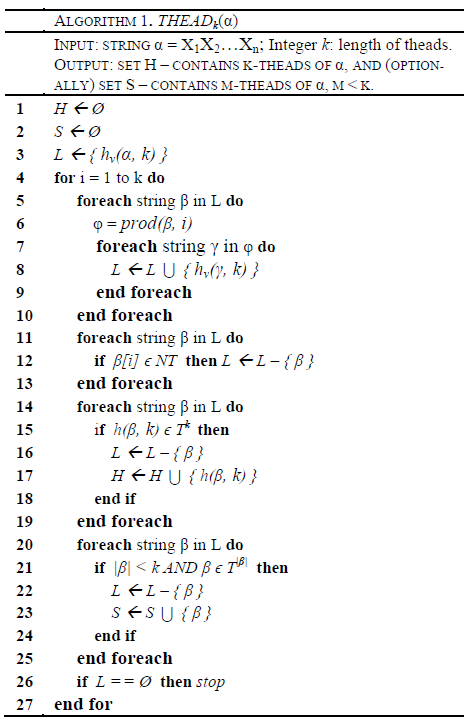
\includegraphics[scale=0.65]{thead_algorithm.PNG}
\caption{Algorithm $THREAD_k(\alpha)$}
\label{fig:thead:algorithm}
\end{figure}

\bigskip
In Algorithm 1, \textbf{H} and \textbf{S} are sets of strings initially empty.
\textbf{L} is an auxiliary ordered list of strings which initially
consists just of $h_v(\alpha, k)$.

Lines 5 to 10 add to the end of L the result of applying
all possible productions to the $i^{th}$ symbol in the current
member $\beta$ of L, omitting strings that are already in L, and
truncating all members added which have k or more symbols
that do not vanish, by deleting the part of the string
following the k-th symbol that does not vanish.

Lines 11 to 13 remove from L all strings whose ith symbol
is a non-terminal.

Lines 14 to 19 remove from L all strings whose prefix of
length k consisting entirely of terminals, and add the prefixes
of length k involved to the set H.

Lines 20 to 25 remove from L all strings of length less
than k which consist entirely of terminals, and add these to
the set S.

On line 26, if L is empty, the algorithm terminates. \textbf{H}
now will contain the required set of terminal strings of
length k of α, i.e., the k-head set of $\alpha$; and S will contain the
set of terminal strings of length less than k which are derived
from $\alpha$. Obviously, \textbf{H} gives the result of $THEAD_k(\alpha)$.

The entire algorithm derives a closure of the initial
string in L, where each derived string in the closure satisfies
the requirements on the length (should be equal to k) of
the strings, and on the type of symbols (should be terminal
symbol) in the strings.


\subsection{Correctness of the Algorithm}
We show the correctness of Algorithm 1 below.

\begin{lemma}
In Algorithm 1, at the end of the $i^{th}$ outer
loop cycle (lines 4-27), for each string s in list L, where s =
$X_1X_2…X_n$, the first i symbols $X1, X2, …, Xi$ of s (or all the
symbols of s if $\mid s \mid < i$) are terminals.
\end{lemma}
\begin{proof}
Prove by induction. For outer loop cycle i = 1, the
step of lines 11-13 removes from L all strings whose $1^{st}$
symbol is a non-terminal. Thus for all the strings remained
in L, the $1^{st}$ symbol is terminal. Now assume at cycle i =
 $n-1$, for all the strings in L, the first i symbols are terminals.
At cycle i = n, the inner loop (lines 5-10) only makes derivations
on the nth symbol, and does not introduce any nonterminal
symbols to the first $n-1$ symbols; next, Algorithm
1 removes from L those strings whose nth symbol is a nonterminal
(lines 11-13), thus for all the symbols in L, now
their first n symbols are terminals. The remaining steps
(lines 14-26) do not alter this fact. Therefore Lemma 1
holds.
\end{proof}

\begin{lemma}
In Algorithm 1, at the end of the $i^{th}$ outer
loop cycle, all the possible combinations of i-thead derivations
are generated by the inner loop (lines 5-10).
\end{lemma}
\begin{proof}
This also can be proved by induction. When i = 1,
this is obvious from the inner loop. Assume this holds for i
= $n-1$. When i = n, for each string s in L, the first $n-1$ symbols
of s are all terminals. In the inner loop, for each string
s in L, all the possible productions are applied to the $n^{th}$
symbol of s, thus all the possible terminal and non-terminal
symbols at the nth position are generated by string s and
included in L. These form new derived strings, appended to
the end of L, and processed by the next cycle. Thus Lemma
2 holds.
\end{proof}

\begin{lemma}
Algorithm 1 ends in k or less outer loop cycles
(lines 4-27) when L becomes empty.
\end{lemma}
\begin{proof}
From Lemma 1, for all the strings generated in
the $k^{th}$ outer loop cycle, their first k symbols are all terminals,
these are then removed from L (lines 14-25). In the
cycles, all members added to L that have k or more symbols
that do not vanish will be truncated (lines 3, 8 and 12).
Thus L will be empty at the end of at most the kth loop
cycle, and Algorithm 1 ends.
\end{proof}

\begin{theorem}
When Algorithm 1 ends, all the possible kthead
derivations are included in H, and all m-thead derivations
are included in S, where $m < k$.
\end{theorem}
\begin{proof}
This follows from Lemma 1, Lemma 2 and
Lemma 3.
\end{proof}


\subsection{Complexity of the Algorithm}
In Algorithm 1, the complexity of the step of lines 6-9 is
$O(|P_{ij}|)$, where $|P_{ij}|$ is the number of possible productions to
the $i^{th}$ symbol in the jth member of L. For the loop of lines
5-10, the complexity is $O(|P_{ij}||L|)$.

The complexity of the entire algorithm is hard to analyze
directly, but it is easy to see that, since the primary output
is set H, the theoretical lower boundary of the number of
steps needed is equal to the number of elements in the output
set: $\Omega(|H|)$. H is the set of terminal strings of length k of
$\alpha$, so $\Omega(|H|)$ = $\Omega(|T|_k)$, where |T| is the number of terminals
in the alphabet. This is the theoretical lower boundary of
both time and space requirements. Obviously, it is exponential
in nature as expected. This is demonstrated by test
case 2 in section 4 “Performance Study”.

\subsection{Comparison with other algorithms}
Aho and Ullman’s method and our method are both
standalone algorithms to compute $FIRST_k(\alpha)$, where the
computation rely on a set of production rules of the grammar
only, and the parsing machine is not needed. Thus
these two methods are better than the other methods in
literature research.

Aho and Ullman’s method takes a bottom up approach
by first calculating $FIRST_i(X)$ for each symbol X, $i = 1, 2,
\ldots k,$ then combining these building blocks to obtain
$FIRST_k(\alpha)$. This is a systematic approach, which is also
demonstrated in their handling of $FIRST_1(\alpha)$, which is
discussed in \cite{aho86compiler}. Once the preparation phase is
done, for whatever input string, the task boils down to
applying the $\oplus_k$ operation on the consisting symbols of
the input string, which concatenates elements from each
set. However, the systematic nature also means that the
overhead must always be taken to achieve good efficiency.
From a practical point of view, since input strings are unknown,
the entire preparation step must be done and its
result be cached for later use.

In comparison, our method takes a top down approach.
No previous computation is needed. The algorithm computes
$FIRST_k(\alpha)$ on the fly based on symbols included in
the input string. No cache is needed. It removes unnecessary
overhead strings on the way of computation.
In nature, both methods are equivalent. Our method can
also be used for the preparation process of Aho and
Ullman’s method.

Another difference is that the $FIRST_k(\alpha)$ method of Aho
and Ullman gives a set of terminal heads whose length $L \leq
k$, and this set must be kept during the entire calculation
process, only at the very end can we remove those $L < k$. In
comparison, our method separates terminal heads into two
sets, for one set the length of terminal heads $L = k$, and for
the other set $L < k$. The second set where $L < k$ can be
ignored from the calculation process.

\section{Examples}
In this section we show how $THEAD_k(\alpha)$ and $FIRST_k(\alpha)$
work on the same input string.

\begin{table}[]
\centering
\caption{Example 4, roud 1 (i=1)}
\label{table:Example4Roud1}
\begin{tabular}{|l|l|l|l|}
\hline	
i & j  & String added to L & String Sequence Number \\
\hline
1 & 1  & XYZU              & 1                      \\
  &    & YYZU              & 2                      \\
  &    & xYZU              & 3                      \\
  &    & YZU               & 4                      \\
  & 2  & ZYZU              & 5                      \\
  &    & yYZU              & 6                      \\
  & 3  &                   &                        \\
  & 4  & ZZU               & 7                      \\
  &    & yZU               & 8                      \\
  &    & ZU                & 9                      \\
  & 5  & zYZU              & 10                     \\
  & 6  &                   &                        \\
  & 7  & XZU               & 11                     \\
  &    & zZU               & 12                     \\
  & 8  &                   &                        \\
  & 9  & XU                & 13                     \\
  &    & zU                & 14                     \\
  &    & U                 & 15                     \\
  & 10 &                   &                        \\
  & 11 & xZU               & 16                     \\
  & 12 &                   &                        \\
  & 13 & YU                & 17                     \\
  &    & xU                & 18                     \\
  & 14 &                   &                        \\
  & 15 & u                 & 19                     \\
  & 16 &                   &                        \\
  & 17 & yU                & 20                     \\
  & 18 &                   &                        \\
  & 19 &                   &                        \\
  & 20 &                   &            \\      
\hline
\end{tabular}
\end{table}

\begin{table}[]
\centering
\caption{Example 4, round 2 (i = 2)}
\label{table:Example4Roud2}
\begin{tabular}{|l|l|l|l|}
\hline
i & j  & String added to L & String Sequence Number \\
\hline
2 &    & xYZU              & 1                      \\
  &    & yYZU              & 2                      \\
  &    & yZU               & 3                      \\
  &    & zYZU              & 4                      \\
  &    & zZU               & 5                      \\
  &    & zU                & 6                      \\
  &    & xZU               & 7                      \\
  &    & xU                & 8                      \\
  &    & yU                & 9                      \\
  & 1  & xZZU              & 10                     \\
  &    & xy                & 11                     \\
  & 2  & yZZU              & 12                     \\
  &    & yy                & 13                     \\
  & 3  & yXU               & 14                     \\
  &    & yz                & 15                     \\
  & 4  & zZZU              & 16                     \\
  &    & zy                & 17                     \\
  & 5  & zXU               & 18                     \\
  &    & zz                & 19                     \\
  & 6  & zu                & 20                     \\
  & 7  & xXU               & 18                     \\
  &    & xz                & 22                     \\
  & 8  & xu                & 23                     \\
  & 9  & yu                & 24                     \\
  & 10 & xXZU              & 25                     \\
  & 11 &                   &                        \\
  & 12 & yXZU              & 25                     \\
  & 13 &                   &                        \\
  & 14 & yYu               & 27                     \\
  &    & yx                & 28                     \\
  & 15 &                   &                        \\
  & 16 & zXZU              & 29                     \\
  & 17 &                   &                        \\
  & 18 & zYU               & 30                     \\
  &    & zx                & 31                     \\
  & 19 &                   &                        \\
  & 20 &                   &                        \\
  & 21 & xYU               & 32                     \\
  &    & xx                & 33                     \\
  & 22 &                   &                       \\
\hline
\end{tabular}
\end{table}

\begin{SampleEnv}

Given grammar G2 ($\epsilon$ is the empty string): 

$X\rightarrow XY | a | \epsilon $

$Y\rightarrow Z | y | \epsilon$

$Z\rightarrow X | z | \epsilon$

$U\rightarrow u$

Find the set of 2-theads of XYZU using 

Algorithm 1:
$THEAD_k(\alpha)$.
\end{SampleEnv}

Since symbols X, Y and Z can all vanish, and U does
not vanish, the string XYZU contains less than 2 symbols
(i.e., only 1) that do not vanish, therefore we need to include
the entire string XYZU as the initial element in the
list L. Thus, at the beginning, L = {XYZU}.

First round of operation for i = 1 is shown in Table ~\ref{table:Example4Roud1}.

At this time, the step of lines 5-10 finishes. Next we follow
lines 11-25. Remove from L all strings with nonterminals
in the ith (first) position; remove from L all
strings whose prefixes of length 2 consisting entirely of
terminals, and add these prefixes to H; and remove from L
all strings of length less than 2 and contains only terminal
strings. At this time, we have H = \{\}, S = \{u\}, L = \{xYZU,
yYZU, yZU, zYZU, zZU, zU, xZU, xU, yU\}.

\hfill

The second round where i = 2 is shown in Table 2.

Remove all strings with non-terminals in the ith (second)
position, remove all strings whose prefixes of length 2 are
made up of terminals, and remove all strings of length less
than 2 and contains only terminal strings, we have H = \{xy,
yy, zy, zz, zu, xu, xz, yz, yx, yu, zx, xx\}, S = \{u\}, L = \{\}.

\begin{SampleEnv}

Given grammar G2 as in Example 3.1, find
the set of 2-theads of XYZU, this time use the $FIRST_k(\alpha)$
algorithm of Aho and Ullman.
\end{SampleEnv}

Following the steps in Aho and Ullman's algorithm, we
need $FIRST_k(\alpha)$, where $\alpha$ = XYZU, and k = 2.

$F_i(p)$ = \{p\}, for all $p \in {x, y, z, u, \epsilon}$, and $i \geq 0$.

$F_0(X) = \{x, \epsilon\}$

$F_0(Y) = \{y, \epsilon\}$

$F_0(Z) = \{z, \epsilon\}$

$F_0(U) = \{u\}$

$F_1(X) = \{x, y, \epsilon\}$

$F_1(Y) = \{y, z, \epsilon\}$

$F_1(Z) = \{z, x, \epsilon\}$

$F_1(U) = \{u\}$

$F_2(X) = \{x, y, z, \epsilon\}$

$F_2(Y) = \{x, y, z, \epsilon\}$

$F_2(Z) = \{x, y, z, \epsilon\}$

$F_2(U) = \{u\}$

\hfill

From this point on $F_i(S) = F_2(S)$ for $i \geq 3$, S = X, Y, Z,
U. It converges here. Therefore:

$FIRST_2(X) = F_2(X) = \{x, y, z, \epsilon\}$

$FIRST_2(Y) = F_2(Y) = \{x, y, z, \epsilon\}$

$FIRST_2(Z) = F_2(Z) = \{x, y, z, \epsilon\}$

$FIRST_2(U) = F_2(U) = \{u\}$

\hfill

Note that here $FIRST_2(X)$ contains strings of length less
than 2, because we need to keep them in the intermediate
steps, as discussed at the end of section 2.4.

Finally, we can calculate $FIRST_k(\alpha) = FIRST_2(XYZU)$
= $FIRST2(X)\oplus_2FIRST_2(Y)\oplus_2 FIRST2(Z)\oplus_2 FIRST_2(U)$
= ${x, y, z, ε}\oplus_2{x, y, z, ε}\oplus_2{x, y, z, ε}\oplus2{u}$
= \{xx, xy, xz, xu, yx, yy, yz, yu, zx, zy, zz, zu, u\}

As a last step as discussed at the end of section 1.3.3, we
remove strings whose length are less than 2, which is 'u'
here, and obtain \{xx, xy, xz, xu, yx, yy, yz, yu, zx, zy, zz,
zu\}. This is the same result as using our algorithm.


\section{Performance Study}
We implemented both the $THEAD_k(\alpha)$ algorithm and the
$FIRST_k(\alpha)$ algorithm, and compared their performance. In
each experiment, the start time and end time are measured
multiple times, and then average start time is subtracted
from average end time to obtain the running time. The
study was conducted on a Sun Microsystems sun4u Netra
440 server running Solaris. CPU is 1.6GHz, memory is 12
GB. For all the experiments below, test case 2 uses the
most memory (hundreds of MB), so memory is not an issue.
In the figure legends, $THEAD$ represents $THEAD_k(\alpha)$,
and $FIRST$ represents $FIRST_k(\alpha)$.

Grammar G2 is used as the testing grammar.

\subsection{Test case 1: $\alpha$ = UUUUUUUUUU, k = 1 to 10}
Result is shown in Table 3 and Figure 2. When α =
UUUUUUUUUU, there is only one terminal head, which is
uk for k = 1 to 10. The speed is very fast, at the level of
microsecond. The relatively long delay when k = 1 for the
$FIRST_k(\alpha)$ algorithm should be caused by the initial construction
of the $F_i(X)$ table.


\begin{table}
\centering
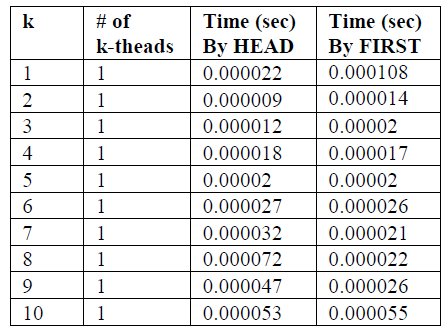
\includegraphics[scale=0.5]{table3.PNG}
\caption{Number of generated k-theads and time spent on
input string UUUUUUUUUU, for k = 1 to 10}
\label{table:3}
\end{table}

\begin{figure}
\centering
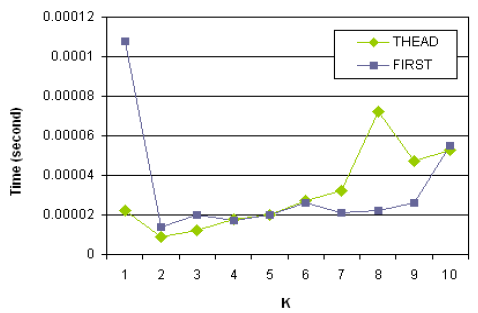
\includegraphics[scale=0.5]{figure2.PNG}
\caption{Time cost of $THEAD_k(\alpha)$ versus $FIRST_k(\alpha)$
for $\alpha$ = UUUUUUUUUU, k = 1 to 10}
\label{fig:2}
\end{figure}


\subsection{Test case 2: $\alpha$ = XXXXXXXXXX, k = 1 to 8}
Result is shown in Table 4 and Figure 3. This is the worst
case scenario where the theoretical bound of exponential
behavior is observed. This is because each symbol of the
input string is a non-terminal (X), which can derive 3 terminals
x, y and z. The number of k-theads that can be generated
is $3^k$. When k is as small as 10, this will take hours to
finish. The result is similar when α = YYYYYYYYYY or
α = ZZZZZZZZZZ.

\begin{table}
\centering
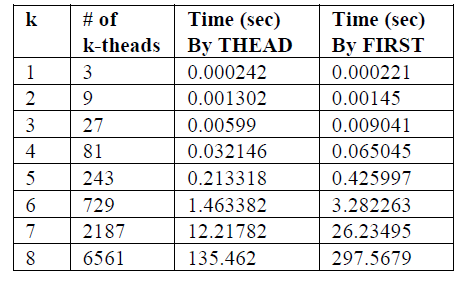
\includegraphics[scale=0.5]{table4.PNG}
\caption{Number of generated k-theads and time spent on
input string XXXXXXXXXX, for k = 1 to 8}
\label{table:4}
\end{table}

\begin{figure}
\centering
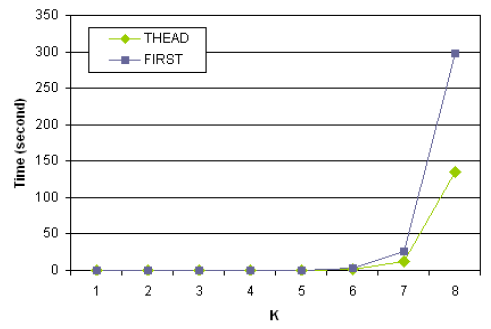
\includegraphics[scale=0.5]{figure3.PNG}
\caption{Time cost of $THEAD_k(\alpha)$ versus $FIRST_k(\alpha)$
for α = XXXXXXXXXX, k = 1 to 8.}
\label{fig:3}
\end{figure}

\subsection{Test case 3: $\alpha$= XYZUXYZUYX, k = 1 to 10}
Result is shown in Table 5 and Figure 4. Here $\alpha$ is a randomly
generated string. We can see that THEADk(α) performs
better than FIRSTk(α) for k = 1 to 9, but for k = 10,
FIRSTk(α) runs faster. This possibly has to do with the way
of implementation: in the implementation of FIRSTk(α), an
ordered list is used to store the strings generated intermediately;
for THEADk(α), the list used cannot be ordered,
since new inserted strings will need to be processed and
have to be attached to the end. When inserting a new generated
string to the end of list L, THEADk(α) will search
through the entire list to make sure it does not exist yet. To
overcome this issue an auxiliary ordered list is used in the
implementation. This slows it down when the list is long.
Of course, better implementation using more efficient data
structure can improve this scenario.

\begin{table}
\centering
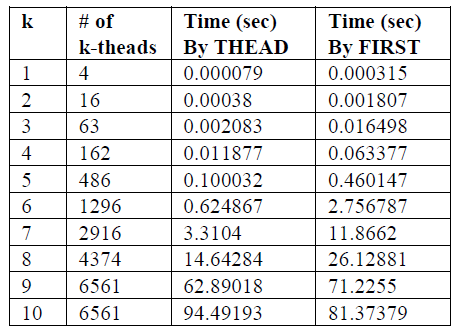
\includegraphics[scale=0.5]{table5.PNG}
\caption{Number of generated k-theads and time spent on
input string XYZUXYZUYX, for k = 1 to 10}
\label{table:5}
\end{table}

\begin{figure}
\centering
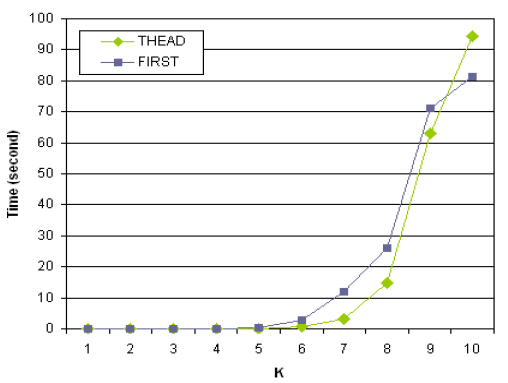
\includegraphics[scale=0.5]{figure4.PNG}
\caption{Time cost of $THEAD_k(\alpha)$ versus $FIRST_k(\alpha)$
for $\alpha$ = XYZUXYZUYX, k = 1 to 10.}
\label{fig:4}
\end{figure}


\subsection{Test case 4: Average on 100 strings of length 10, k
= 1 to 8}
100 input strings, each of length 10, are generated from the
alphabet of {X, Y, Z, U} using a random number generator,
and then fed to the algorithms to compare their performance.
This means the input strings may be like:
\begin{tabular}{ll}
1   & YXXXYUUUUU                                                                                                   \\
2   & UZZUUUZXXY                                                                                                  \\
3   & YZZUYZZYZU                                                                                                \\
4   & ZZUZUZYUZY                                                                                                \\
    & ....                                                                                                \\
100 &UUYXXUUXUY \\
\end{tabular}

Result is shown in Table 6 and Figure 5. Table 6 shows
the average number of k-theads generated and average time
used by the $THEAD_k(\alpha)$ and $FIRST_k(\alpha)$ algorithms over
100 input strings of length 10, and k = 1 to 8. Figure 5
shows the graphical version of the average time used when
k increases. It can be seen that the $THEAD_k(\alpha)$ algorithm
uses less time.

\begin{table}
\centering
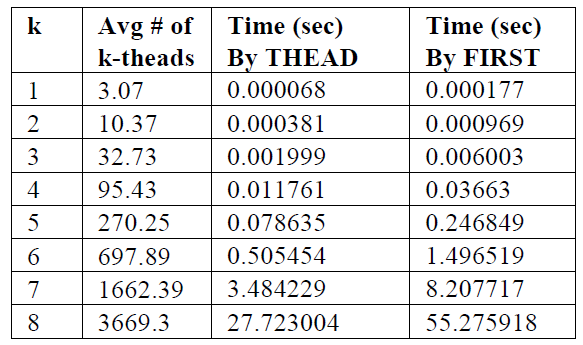
\includegraphics[scale=0.5]{table6.PNG}
\caption{Average number of generated k-theads and time
spent on 100 random strings of length 10, for k = 1 to 8}
\label{table:6}
\end{table}

\begin{figure}
\centering
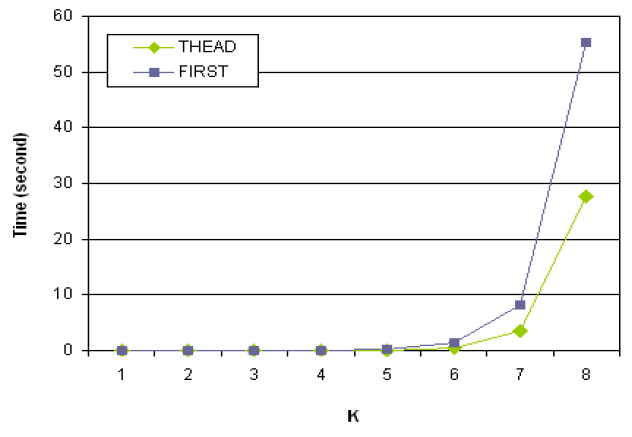
\includegraphics[scale=0.5]{figure5.PNG}
\caption{Time cost of $THEAD_k(\alpha)$ versus $FIRST_k(\alpha)$
fwhen k increases. Averaged over 100 strings of length 10}
\label{fig:5}
\end{figure}


\subsection{Test case 5: 100 strings of length 1 to 100, k = 2}
In this test case, k is fixed, while the input string is a kprefix
of the following randomly generated string, where
input string length $|\alpha|$ = 1 to 100, i.e., the input strings may
be like:\\
\begin{tabular}{ll}
1   & Y                                                                                                   \\
2   & YZ                                                                                                  \\
3   & YZZ                                                                                                 \\
4   & YZZY                                                                                                \\
    & ....                                                                                                \\
100 & YZZYYXZYYXYZUXYYUYXZUYYUZXUYZZ \\
      & YYZXXXXXUUUYXYZZYZYZUUXZXZYZXX \\
      & UZUXYZYYYUYZZZZZUZXZYYYYZYYUXZ \\
      & ZUYZUZXUY
\end{tabular}


\begin{figure}
\centering
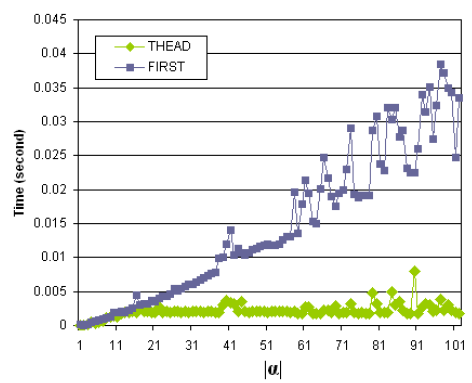
\includegraphics[scale=0.5]{figure6.PNG}
\caption{Time cost of $THEAD_k(\alpha)$ versus $FIRST_k(\alpha)$
when k = 2, and string length $|\alpha|$ increases}
\label{fig:6}
\end{figure}

%TODO
\subsection{Summary}
We can draw several conclusions from the experiments.

First of all, when the input string contains terminal symbols
only, the speed is the fastest. When the input string
contains non-terminal symbols only, the speed is the slowest,
and may lead to the worst case scenario: exponential
increase in computation time. For a grammar as simple as
G2, when k = 10, it will take hours to finish using both
algorithms.

In general the $THEAD_k(\alpha)$ algorithm performs better
than the $FIRST_k(\alpha)$ algorithm, as shown by test case 4,
which is averaged over 100 randomly generated strings of
length 10 for k = 1 to 10.

However, it is also possible that $FIRST_k(\alpha)$ runs faster
than $THEAD_k(\alpha)$, as shown in test case 3 when k = 10.
Finally, when k is small, but input string is long,
$THEAD_k(\alpha)$ will perform better than $FIRST_k(\alpha)$, as shown
by test case 5. Actually, for this scenario, the time
$THEAD_k(\alpha)$ takes will not increase when the size of the
input string increase. However, the time used by $FIRST_k(\alpha)$
will increase linearly according to the length of the input
string.

\section{Implementation}
We briefly discuss the implementation of the two approaches
here, which is done in ANSI C from scratch.

To make the comparison of the two algorithms reasonable,
it is necessary to implement them with similar data
structures.

The major operations involved in both algorithms are set
operations. In the current implementation, a set is implemented
as a linked list. Search in the set is done by going
through the list in linear order. That a linked list is chosen
for the implementation is because of the nature of the
THEADk(α) algorithm: a new generated string has to be
appended to the end of the current set, which makes queue
a natural and necessary choice. A queue of unknown size as
in the current scenario is in turn naturally implemented as a
linked list.

To guarantee similar search experience for both algorithms,
an ordered list is used. For the method of Aho and
Ullman, this is no problem. But for the THEADk(α) method,
the queue (implemented as a list) to be appended to can
not be ordered, so an auxiliary list is provided which stores
the same strings as the queue but is in sorted order, such
that when a search in the auxiliary ordered list does not
return a hit, the new string is appended to the end of the
queue. The maintenance of two lists in the THEADk(α)
algorithm implementation obviously will slow it down to
some degree.

This implementation can be improved by providing an
auxiliary binary search tree or a hash table to both methods,
which works much more efficient when decide if a string
exists in a set. This improvement should be of more significance
to the performance of the THEADk(α) algorithm
implementation according to the above discussion.

Finally, a linked list suffices for all the operations of the
THEADk(α) algorithm. For the algorithm of Aho and
Ullman, an array is also used to store the pre-computed
FIRSTk(Xi) values of all the symbols Xi, such that given a
random string α = X1X2…Xn, FIRSTk(Xi) can be retrieved
in constant time using index of Xi in the symbol table for
the calculation of FIRSTk(α) = $FIRST_k(X_1)\oplus_k$
$FIRST_k(X_2)$ $\oplus_k …\oplus_k FIRST_k(X_n)$.

\section{Application}
One application of the algorithm presented here is to be
used in a LR(k) parser generation algorithm.

Our study of the LR(k) algorithm shows that the calculation
of LR(k) lookahead is one of the major steps involved.
We designed and implemented the Edge-Pushing LR(k)
algorithm, which depends on the THEADk(α) function to
calculate k-lookahead. The Edge-Pushing algorithm is
shown below in Figure 7, which is taken from a previous
paper [11]. The THEADk(α) algorithm is used on line 13.

The Edge-Pushing algorithm is implemented in the
HYACC parser generator, which is available as an open
source parser generator [12][13].

\section{Conclusion}
In this paper we have presented a new algorithm to calculate
the terminal heads of length k, which is called
THEADk(α).

We reviewed relevant literature, of which Aho and
Ullman’s method is the only previously available
standalone algorithm for this purpose.
We showed the new algorithm, discussed its correctness
and complexity, and compared to previous work. Examples
are given to evaluate terminal heads of length k of a given
string by using the THEADk(α) algorithm and the
FIRSTk(α) method of Aho and Ullman.

An empirical study was conducted to compare the
THEADk(α) algorithm and the FIRSTk(α) algorithm. In
general, when averaged over a large number of randomly
generated input strings, THEADk(α) performs faster than
FIRSTk(α). When the input string α is long but k is small,
THEADk(α) always performs better than FIRSTk(α).

Finally, we discussed the application of the new
THEADk(α) algorithm, and pointed out that it has been
used to implement the edge-pushing algorithm in the HYACC
parser generator.

Due to the fact that FIRSTk(α) is a fundamental algorithm
that works as a basic building block in compiler theory
and practice, its improvement should have wide impact.


%
% The following two commands are all you need in the
% initial runs of your .tex file to
% produce the bibliography for the citations in your paper.
\bibliographystyle{abbrv}
\bibliography{sigproc}  % sigproc.bib is the name of the Bibliography in this case
% You must have a proper ".bib" file
%  and remember to run:
% latex bibtex latex latex
% to resolve all references
%
% ACM needs 'a single self-contained file'!
%
%APPENDICES are optional
%\balancecolumns

\end{document}
